\section{Single-Task Neural Networks Results}
\label{sec:single_results}
In this Section we report the results obtained using single-tasks neural networks. Since this deep learning model is considered the state-of-the-art in CRRs classification, we use these experiments as a benchmark for evaluating the performance of multi-task neural networks (Section~\ref{sec:multi_results}). The experiments are performed with the experimental setups described in Section~\ref{sec:exp_setup_general} and Section~\ref{sec:exp_setup_singletask}, the model are trained using the two set of features described in Section~\ref{sec:featureselection} 

Firstly, we discuss the results obtained training a single-task neural network using $F_\ell^{\textrm{acc}}$ as features set and without balancing the dataset. The bar plots in Figure~\ref{fig:unbalanced_old_results} report the average auROC and auPRC obtained, the same results are summarized in Table~\ref{tab:unbalanced_old_auroc} and Table~\ref{tab:unbalanced_old_auprc} in Appendix~\ref{appendix:results_tables}. Almost for every computational tasks auROC is greater than 0.6. Despite this in some cases, such as A-P vs I-P and I-E vs I-P respectively in HEK293 and MCF7, the model obtained very low results. auPRC results instead are not very promising. In both average auROC and average auPRC results emerge that this model is very good in distinguish active enhancers from active promoters (A-E vs A-P) obtaining always values greater than 0.9.
\begin{figure}[!htbp]
    \centering
    \begin{subfigure}[b]{\textwidth}
        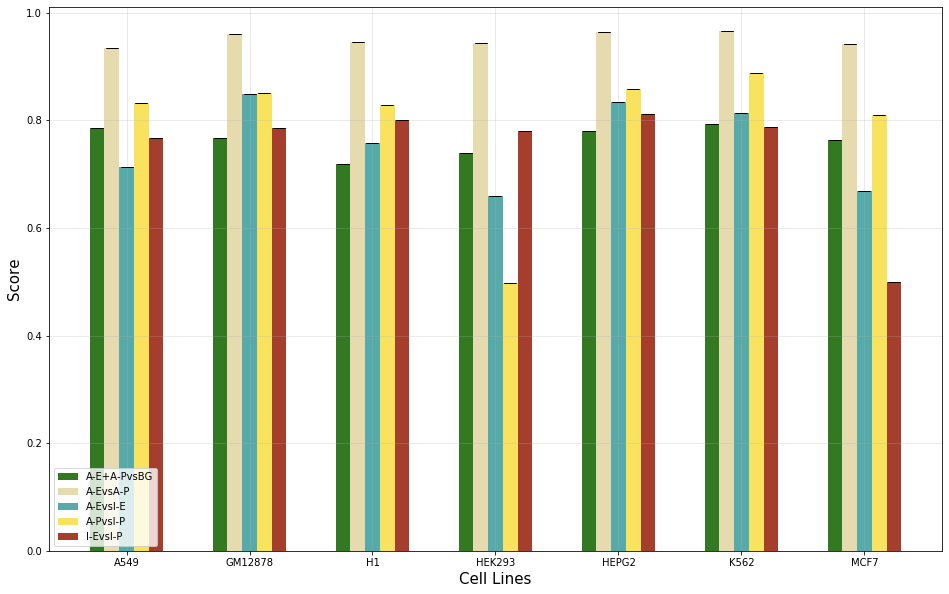
\includegraphics[width=\textwidth]{images/results_plots/single_tasks/unbalanced_old_auroc.png}
        \caption{auROC}
        \label{fig:auroc_unbalanced_old}
    \end{subfigure}
    \begin{subfigure}[b]{\textwidth}
        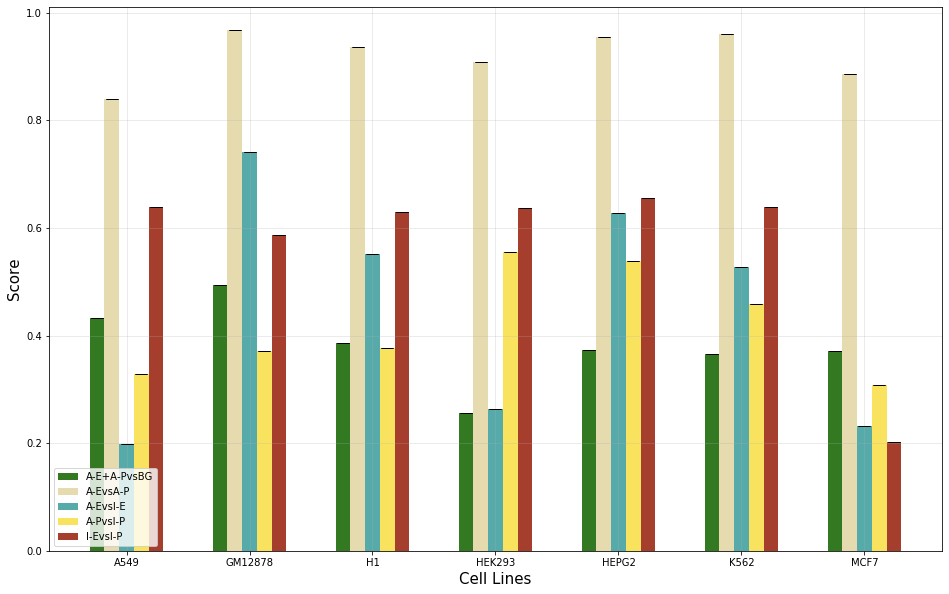
\includegraphics[width=\textwidth]{images/results_plots/single_tasks/unbalanced_old_auprc.png}
        \caption{auPRC}
        \label{fig:auprc_unbalanced_old}
    \end{subfigure}
    \caption{auROC and auPRC for single-task neural network trained using $F_\ell^{\textrm{acc}}$ as features and unbalanced dataset.}\label{fig:unbalanced_old_results}
\end{figure}

In order to improve the results of the model, using the same set of features $F_\ell^{\textrm{acc}}$, we repeated the experiment balancing both training and test set. Comparing Figure~\ref{fig:auprc_balanced_old}, containing the results with a balanced dataset, and Figure~\ref{fig:auroc_unbalanced_old}, containing the previous results with unbalanced setting, we can notice an average auPRC improvement in almost every tasks $p$ of every cell lines $\ell \in L$. On the other hand the average auROC remains nearly unchanged (Figure~\ref{fig:balanced_old_results} and Figure~\ref{fig:unbalanced_old_results}). 

\begin{figure}[!htbp]
    \centering
    \begin{subfigure}[b]{\textwidth}
        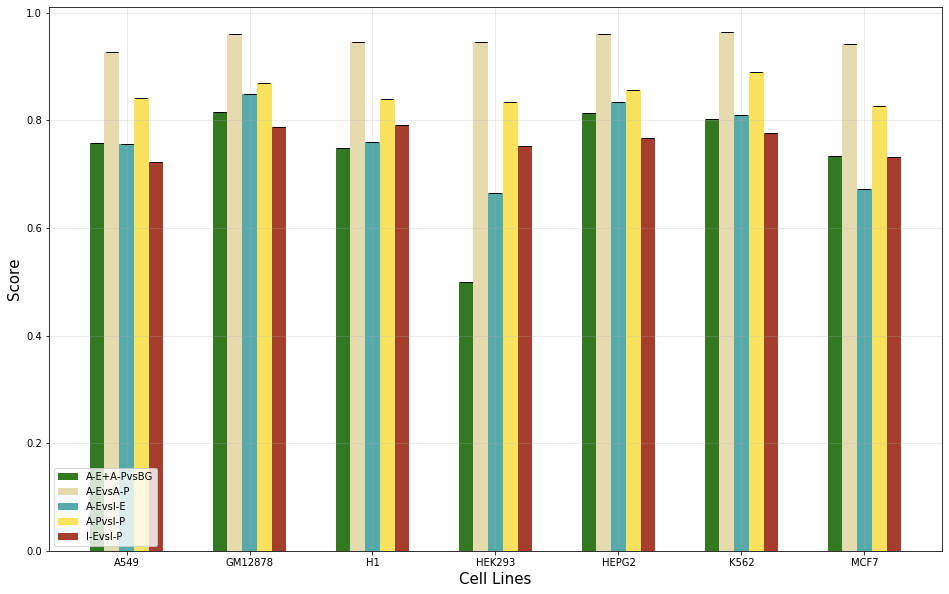
\includegraphics[width=\textwidth]{images/results_plots/single_tasks/balanced_old_auroc.png}
        \caption{auROC}
        \label{fig:auroc_balanced_old}
    \end{subfigure}
    \begin{subfigure}[b]{\textwidth}
        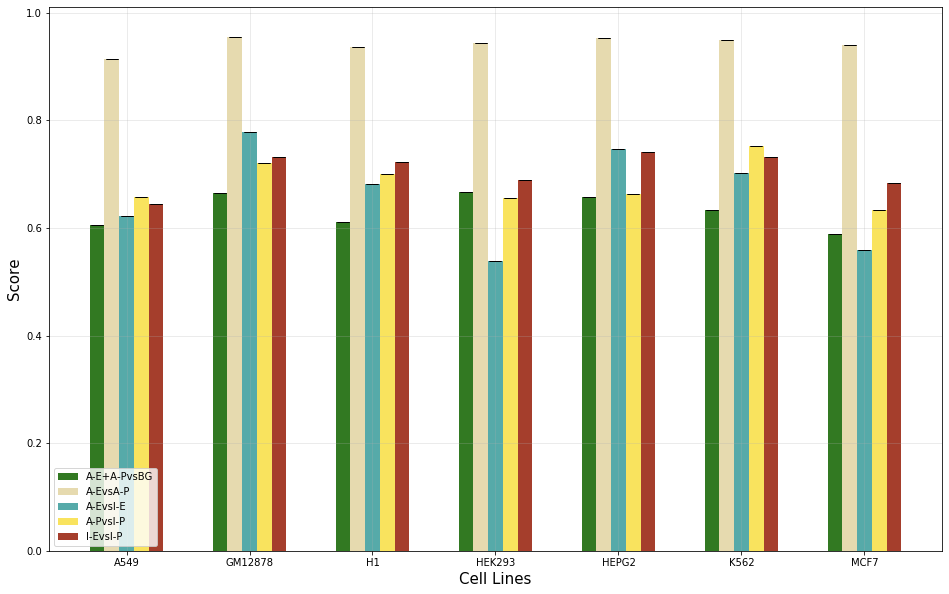
\includegraphics[width=\textwidth]{images/results_plots/single_tasks/balanced_old_auprc.png}
        \caption{auPRC}
        \label{fig:auprc_balanced_old}
    \end{subfigure}
    \caption{auROC and auPRC for single-task neural network trained using $F_\ell^{\textrm{acc}}$ as features and balanced dataset.}\label{fig:balanced_old_results}
\end{figure}

Finally, we repeated the experiments using the set of features selected using f1-score $F_\ell^{\textrm{f1}}$. Both for balanced and unbalanced dataset the results are similar compared to the features selected using accuracy. the best results are always obtained using a balanced dataset configuration to train the model. The bar plot of average auROC and average auPRC of these experiments are reported in Figure~\ref{fig:unbalanced_new_results} and Figure~\ref{fig:balanced_new_results}, the numerical values are summarized in Table~\ref{tab:unbalanced_new_auroc} and Table~\ref{tab:unbalanced_new_auprc} for the unbalanced dataset, Table~\ref{tab:balanced_new_auroc} and Table~\ref{tab:balanced_new_auprc} instead report the values for the balanced. 

\begin{figure}[!htbp]
    \centering
    \begin{subfigure}[b]{\textwidth}
        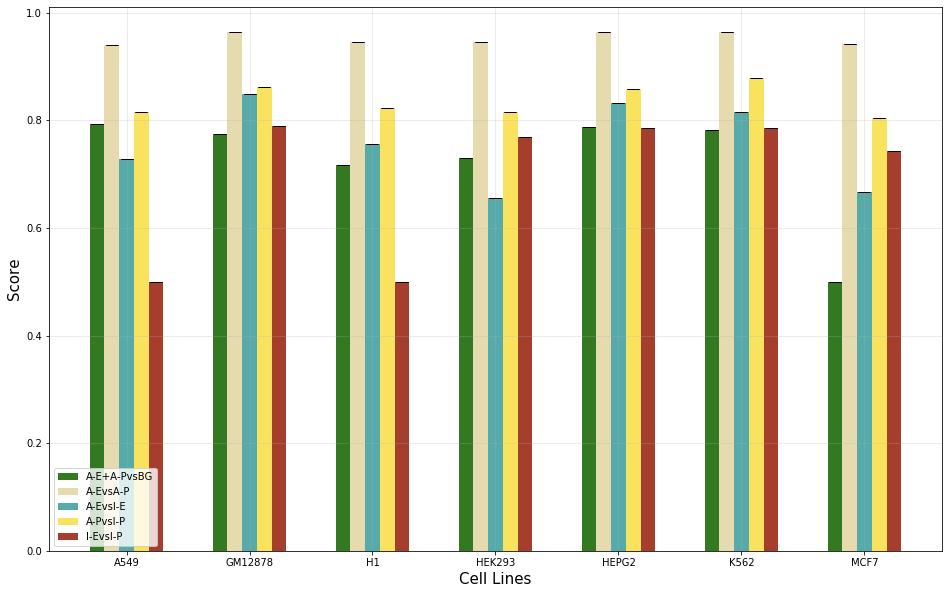
\includegraphics[width=\textwidth]{images/results_plots/single_tasks/unbalanced_new_auroc.png}
        \caption{auROC}
        \label{fig:auroc_unbalanced_new}
    \end{subfigure}
    \begin{subfigure}[b]{\textwidth}
        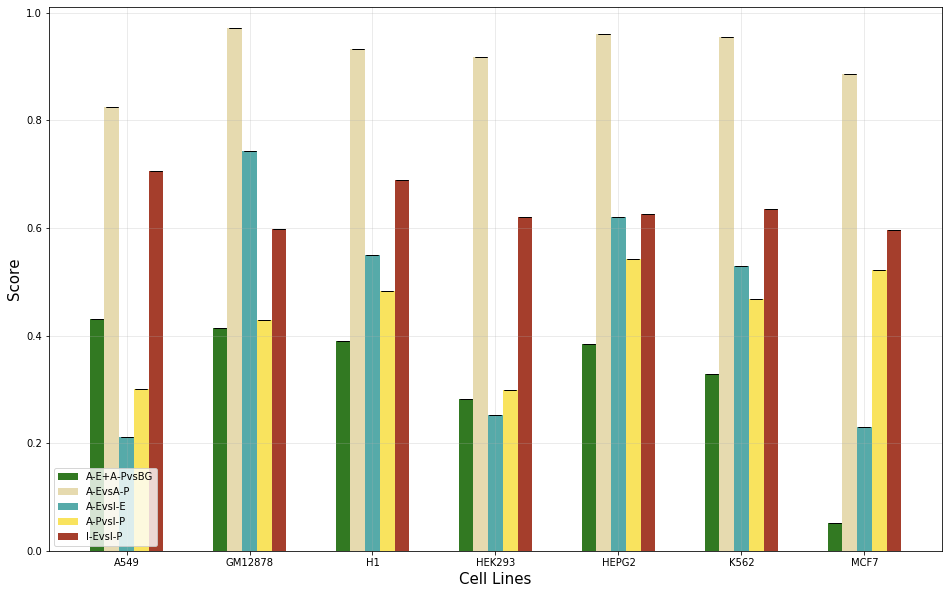
\includegraphics[width=\textwidth]{images/results_plots/single_tasks/unbalanced_new_auprc.png}
        \caption{auPRC}
        \label{fig:auprc_unbalanced_new}
    \end{subfigure}
    \caption{auROC and auPRC for single-task neural network trained using $F_\ell^{\textrm{f1}}$ as features and unbalanced dataset.}\label{fig:unbalanced_new_results}
\end{figure}

\begin{figure}[!htbp]
    \centering
    \begin{subfigure}[b]{\textwidth}
        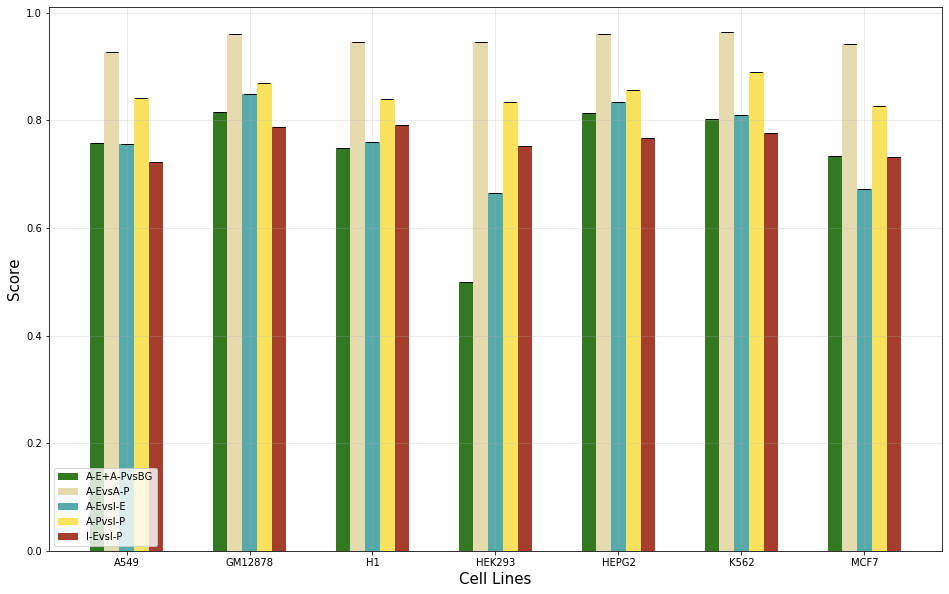
\includegraphics[width=\textwidth]{images/results_plots/single_tasks/balanced_new_auroc.png}
        \caption{auROC}
        \label{fig:auroc_balanced_new}
    \end{subfigure}
    \begin{subfigure}[b]{\textwidth}
        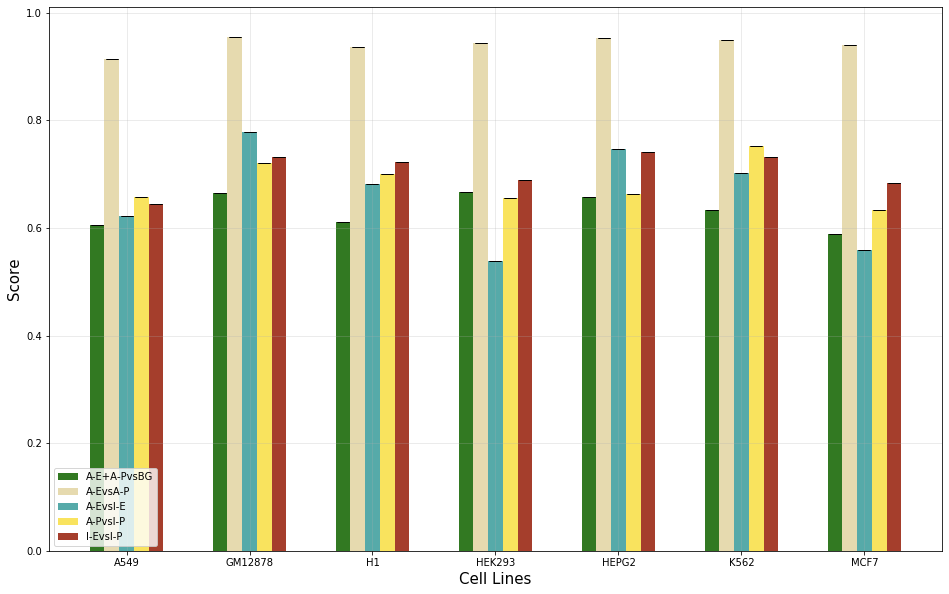
\includegraphics[width=\textwidth]{images/results_plots/single_tasks/balanced_new_auprc.png}
        \caption{auPRC}
        \label{fig:auprc_balanced_new}
    \end{subfigure}
    \caption{auROC and auPRC for single-task neural network trained using $F_\ell^{\textrm{f1}}$ as features and balanced dataset.}\label{fig:balanced_new_results}
\end{figure}

\section{Multi-Task Neural networks results} \label{sec:multi_results}
In this Section we report the results obtained from various experiments performed with the aim to evaluate multi-task neural networks (Section~\ref{sec:MTLsection}) in CRRs classification. We trained the models using different experimental setups explained in Section~\ref{sec:exp_setup_general} and Section~\ref{sec:exp_setup_multitask}. Furthermore, we used both $F_\ell^{\textrm{acc}}$ and $F_\ell^{\textrm{f1}}$ features sets, selected using respectively accuracy and f1-score (Section~\ref{sec:featureselection}).

Initially, the experiments were performed with the first set of features, $F_\ell^{\textrm{acc}}$, and with a fixed number of neurons. In Table~\ref{tab:fixed_neurons_auroc} and Table~\ref{tab:fixed_neurons_auprc} we reported the averages of auROC and auPRC of every holdouts with the corresponding standard deviation (STD). In Figure~\ref{fig:fixed_neurons_results} we show the same results visually for an easier comparison. Apart some exceptions, such as I-P vs I-E or A-E vs I-E in HEPG2 and GM12878, looking at Figure~\ref{fig:auprc_fixed_neurons} we can notice that we often have a very low auPRC. 
\begin{figure}[!htbp]
    \centering
    \begin{subfigure}[b]{\textwidth}
        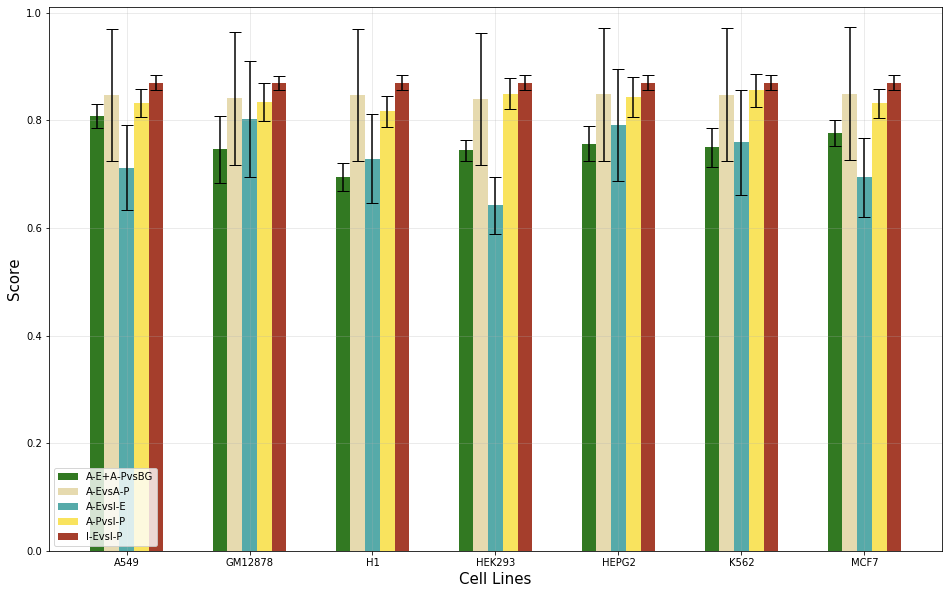
\includegraphics[width=\textwidth]{images/results_plots/fixed_neurons_auroc.png}
        \caption{auROC}
        \label{fig:auroc_fixed_neurons}
    \end{subfigure}
    \begin{subfigure}[b]{\textwidth}
        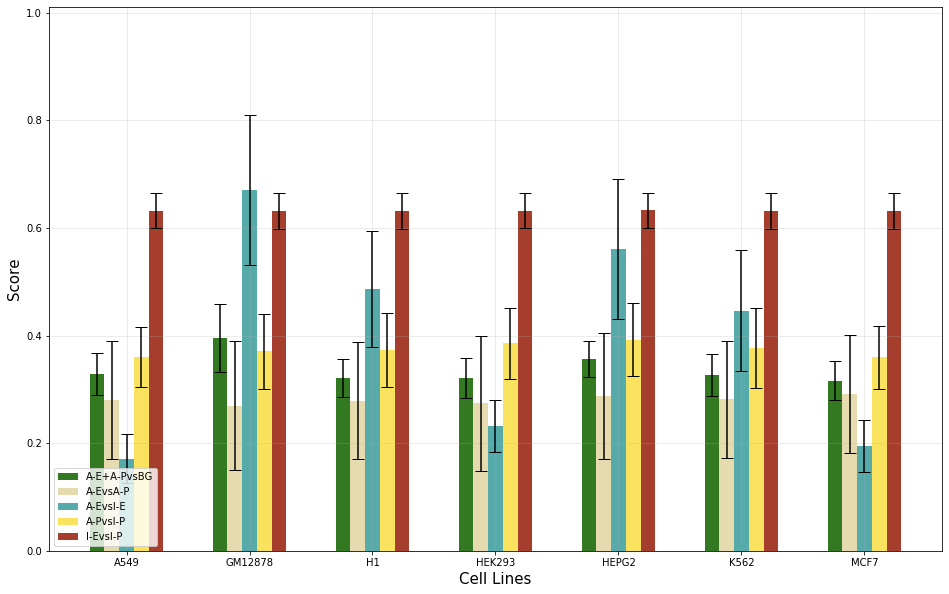
\includegraphics[width=\textwidth]{images/results_plots/fixed_neurons_auprc.png}
        \caption{auPRC}
        \label{fig:auprc_fixed_neurons}
    \end{subfigure}
    \caption{auROC and auPRC for multi-tasks neural network trained using $F_\ell^{\textrm{acc}}$, fixed size of neurons and unbalanced dataset.}
    \label{fig:fixed_neurons_results}
\end{figure}

In order to improve the performance of the models we tried to balance both training and test set. In Figure~\ref{fig:balanced_results} we reported the bar plots for average auROC (Figure~\ref{fig:auroc_balanced}) and average auPRC (Figure~\ref{fig:auprc_balanced}). Furthermore, in Table~\ref{tab:balanced_auroc} and Table~\ref{tab:balanced_auprc} we summarized the numerical values. We can notice that a performance increase is shown in both auROC and auPRC results. In particular in every cell line $\ell \in L$ and every computational task $p$, excluding A-E vs A-P that remain almost 0.1, we have a noticeable improvement in auPRC.  
%
\begin{figure}[!htbp]
    \centering
    \begin{subfigure}[b]{\textwidth}
        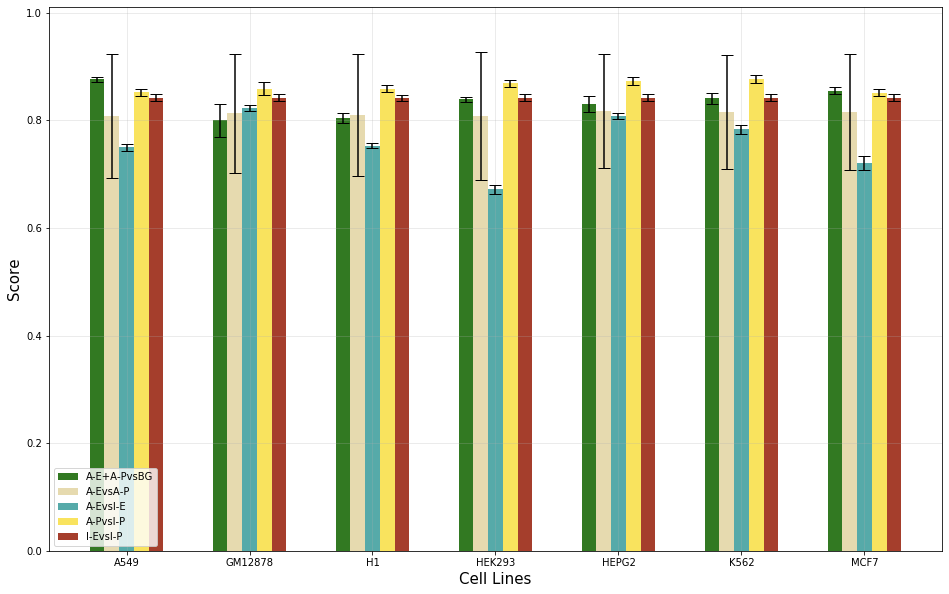
\includegraphics[width=\textwidth]{images/results_plots/balanced_dataset_auroc.png}
        \caption{auROC}
        \label{fig:auroc_balanced}
    \end{subfigure}
    \begin{subfigure}[b]{\textwidth}
        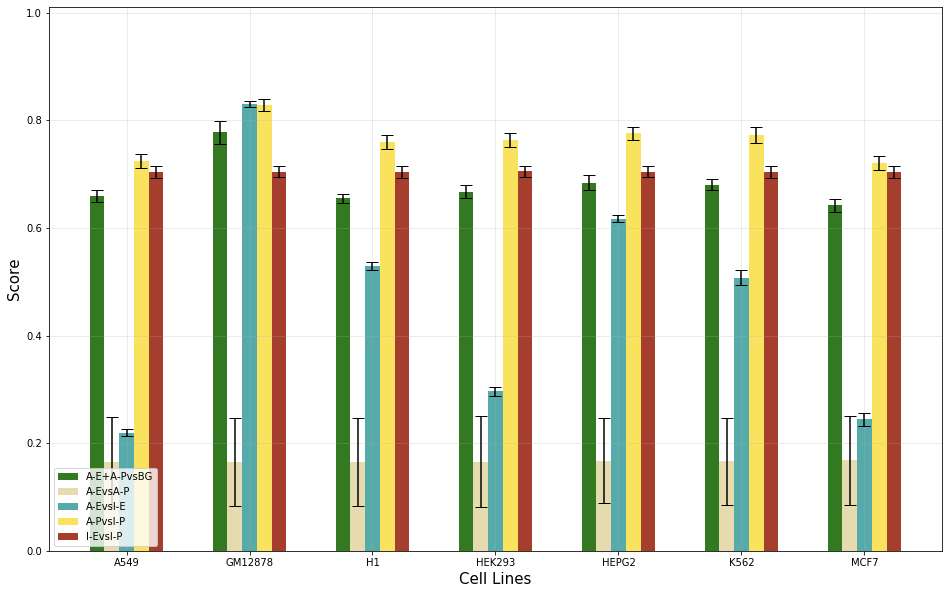
\includegraphics[width=\textwidth]{images/results_plots/balanced_dataset_auprc.png}
        \caption{auPRC}
        \label{fig:auprc_balanced}
    \end{subfigure}
    \caption{auROC and auPRC for multi-tasks neural network trained using $F_\ell^{\textrm{acc}}$, fixed size of neurons and balanced dataset.}
    \label{fig:balanced_results}
\end{figure}

Another experiment performed using $F_\ell^{\textrm{acc}}$ set is the one using a pyramidal architecture. We choose to maintain the dataset balanced due to the good performance highlighted. Overall, compared to the the previous fixed neurons configuration no particular performance improvement emerge using this configuration. The auROC bar plot in Figure~\ref{fig:auroc_pyramydal} shows a slight improvement compared to Figure~\ref{fig:auroc_balanced}. Looking at auPRC values we can notice that there are clear improvements for some tasks, such as A-E vs I-E in MCF7, but a huge decrease for some cell lines (i.e., A549, H1). The results obtained are reported in Figure~\ref{fig:pyramydal_results} and the values summarized in Table~\ref{tab:pyramidal_auroc} and Table~\ref{tab:pyramidal_auprc} in Appendix~\ref{appendix:results_tables}. The standard deviations in both auROC and auPRC has decreased significantly.  
%%
\begin{figure}[!htbp]
    \centering
    \begin{subfigure}[b]{\textwidth}
        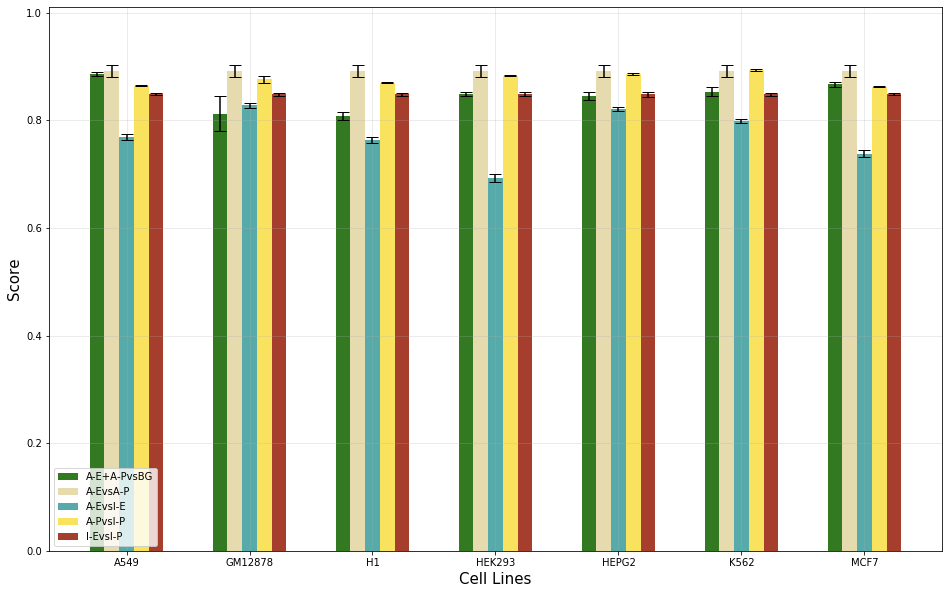
\includegraphics[width=\textwidth]{images/results_plots/pyramydal_auroc.png}
        \caption{auROC}
        \label{fig:auroc_pyramydal}
    \end{subfigure}
    \begin{subfigure}[b]{\textwidth}
        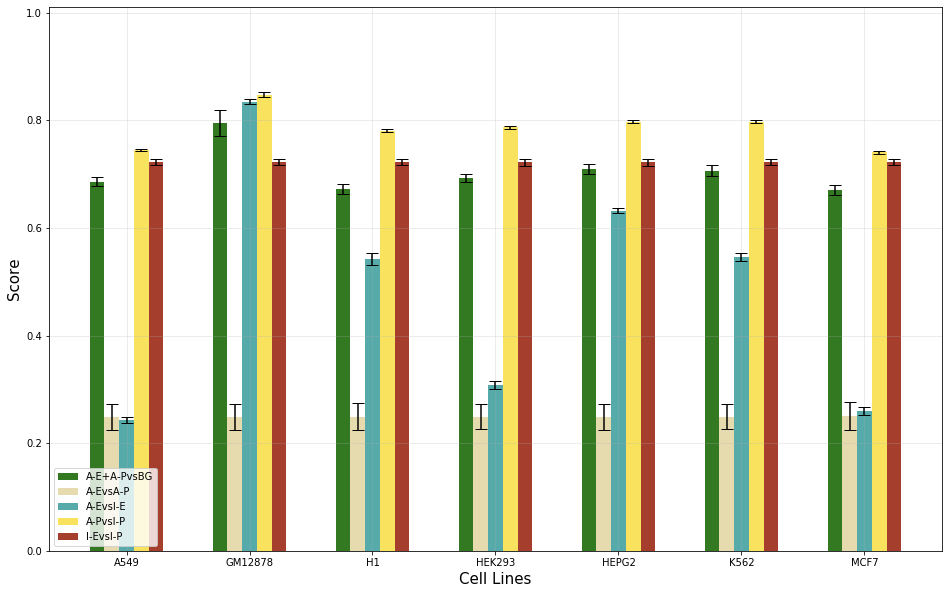
\includegraphics[width=\textwidth]{images/results_plots/pyramydal_auprc.png}
        \caption{auPRC}
        \label{fig:auprc_pyramydal}
    \end{subfigure}
    \caption{auROC and auPRC for multi-tasks neural network trained using $F_\ell^{\textrm{acc}}$, pyramidal structure and balanced dataset.}\label{fig:pyramydal_results}
\end{figure}
%%

In order to test whether the number of tasks influence the performance of the model we tried to reduce it from seven to four. The idea is that with many tasks could be harder for the model to share knowledge. For those reasons for the last experiment performed on the first set of features we reduced the set of cell lines $L$ to GM12878, A549, HEPG2 and K562. In Figure~\ref{fig:4celllines_results} we report the average auROC and auPRC obtained, the values are summarized in Table~\ref{tab:4celllines_auprc} and Table~\ref{tab:4celllines_auroc} of Appendix~\ref{appendix:results_tables}. The results shows a significant improvement. The average auROC (Figure~\ref{fig:auroc_4celllines}) is greater than 0.8 for every task and every cell lines, sometimes even higher than 0.95. For auPRC bar plot instead we can see an improvement in many tasks compared to the previous experiments.
%%
\begin{figure}[!htbp]
    \centering
    \begin{subfigure}[b]{\textwidth}
        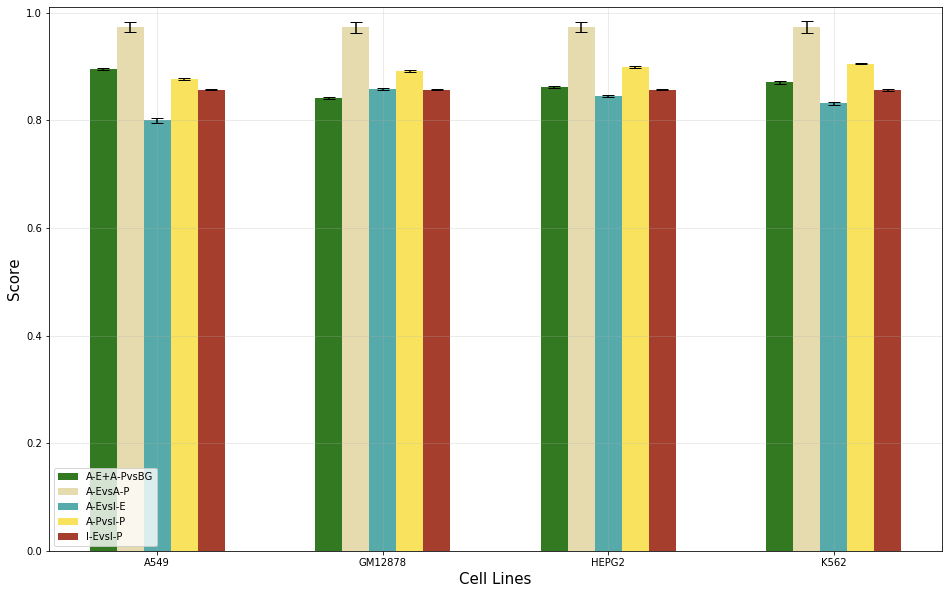
\includegraphics[width=\textwidth]{images/results_plots/4celllines_auroc.png}
        \caption{auROC}
        \label{fig:auroc_4celllines}
    \end{subfigure}
    \begin{subfigure}[b]{\textwidth}
        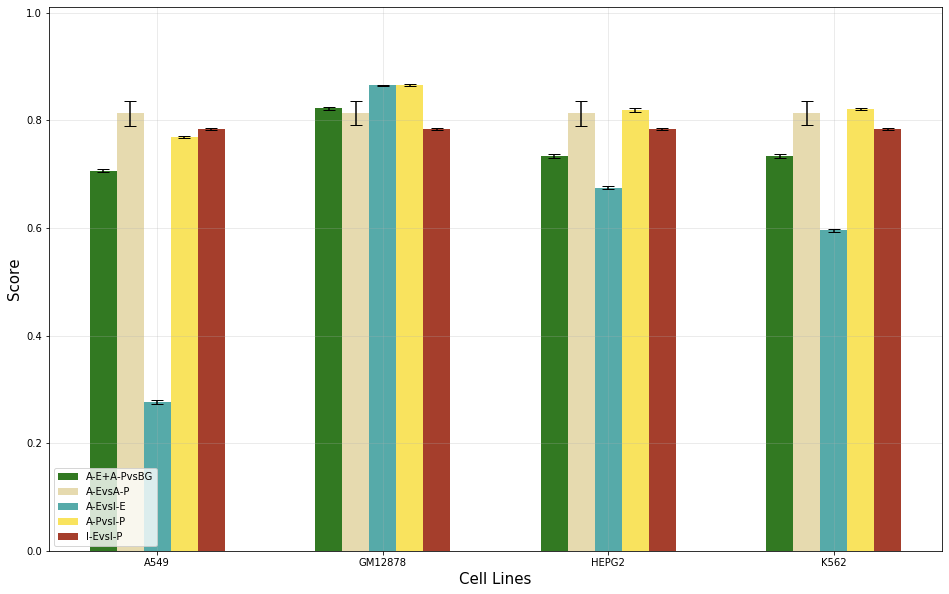
\includegraphics[width=\textwidth]{images/results_plots/4celllines_auprc.png}
        \caption{auPRC}
        \label{fig:auprc_4celllines}
    \end{subfigure}
    \caption{auROC and auPRC for multi-tasks neural network trained using $F_\ell^{\textrm{acc}}$, reduced number of tasks and balanced dataset.}
    \label{fig:4celllines_results}
\end{figure}

Regarding the second set of features $|F_\ell^{\textrm{f1}}|$, chosen using f1-score as evaluating metric, we performed two experiments. The former with neural network pyramidal structure and unbalanced training and test sets, the latter using the same sets of reduced tasks used in the previous experiment (GM12878, A549, HEPG2 and K562) with balanced dataset. 
\begin{figure}[!htbp]
    \centering
    \begin{subfigure}[b]{\textwidth}
        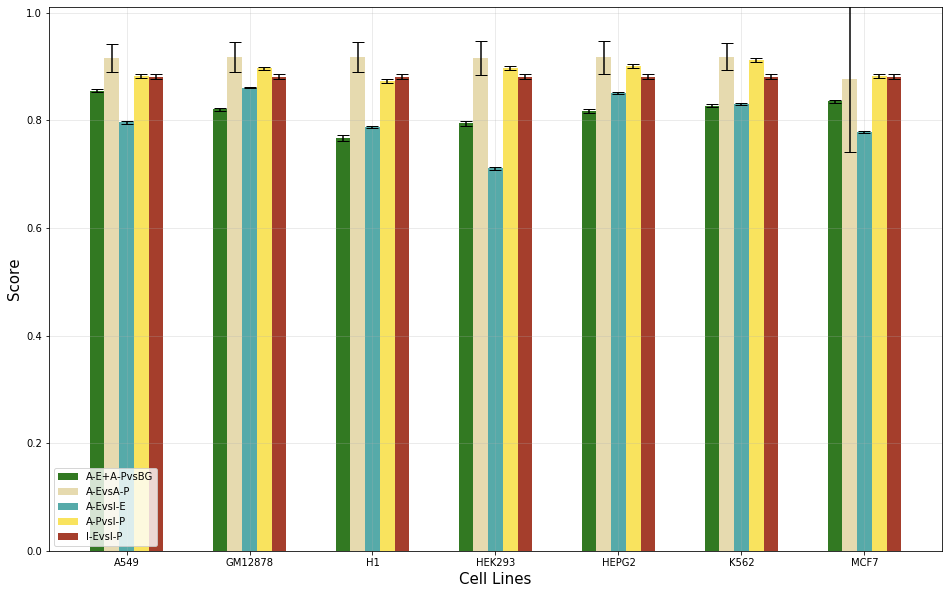
\includegraphics[width=\textwidth]{images/results_plots/new_features_auroc.png}
        \caption{auROC}
        \label{fig:auroc_newfeatures}
    \end{subfigure}
    \begin{subfigure}[b]{\textwidth}
        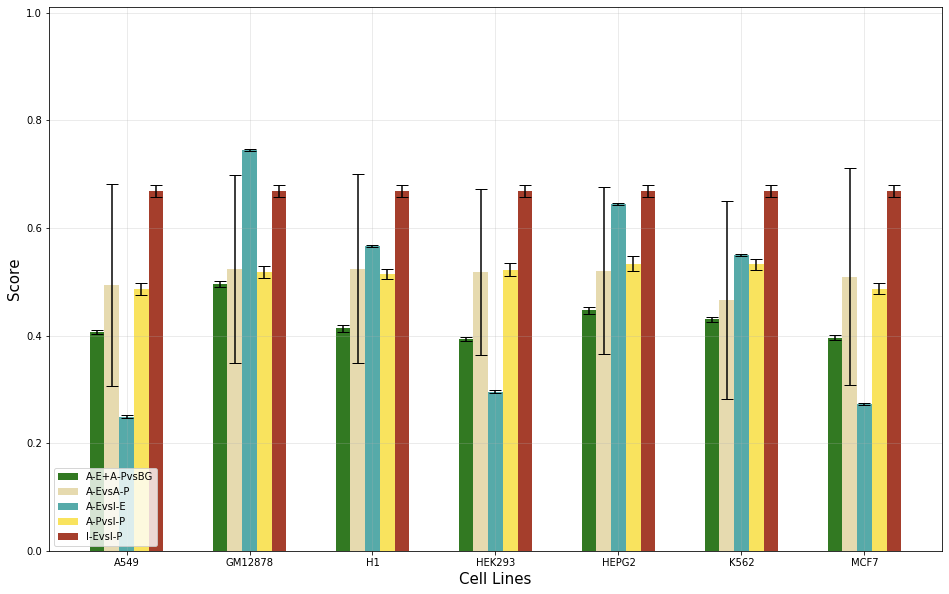
\includegraphics[width=\textwidth]{images/results_plots/new_features_auprc.png}
        \caption{auPRC}
        \label{fig:auprc_newfeatures}
    \end{subfigure}
    \caption{auROC and auPRC for multi-tasks neural network trained using $F_\ell^{\textrm{f1}}$, pyramidal structure and unbalanced dataset.}\label{fig:newfeatures_results}
\end{figure}
%%
\begin{figure}[!htbp]
    \centering
    \begin{subfigure}[b]{\textwidth}
        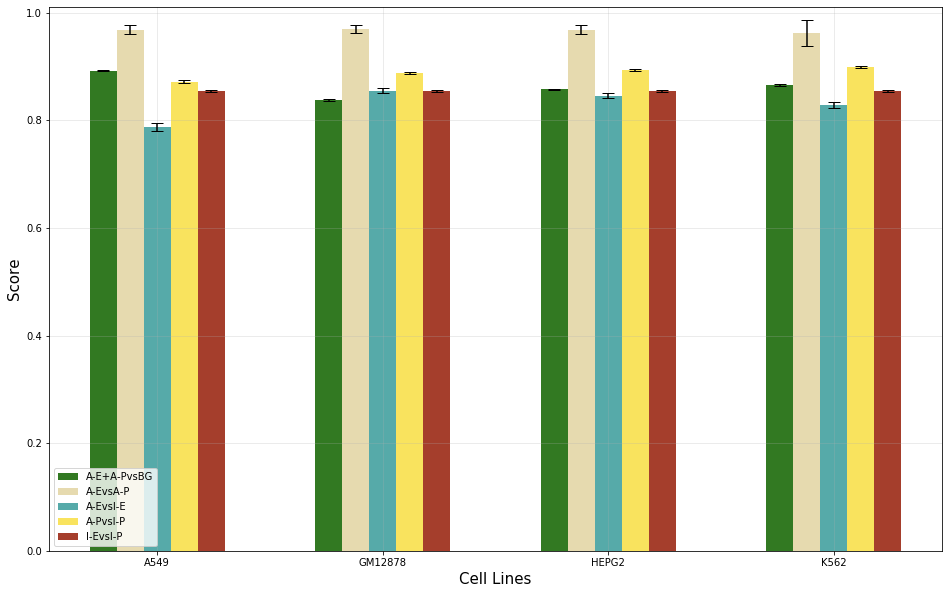
\includegraphics[width=\textwidth]{images/results_plots/4celllines_new_auroc.png}
        \caption{auROC}
        \label{fig:auroc_new_4celllines}
    \end{subfigure}
    \begin{subfigure}[b]{\textwidth}
        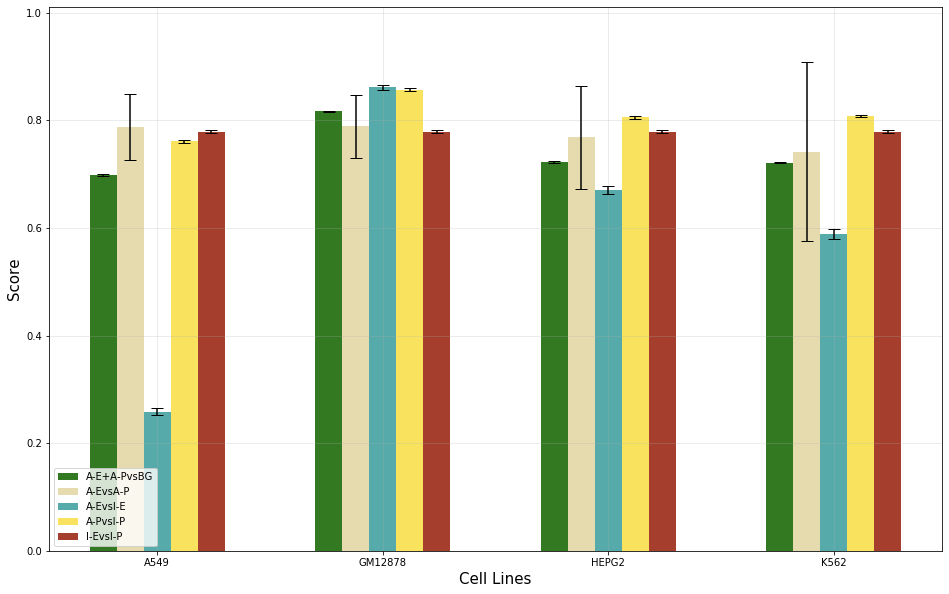
\includegraphics[width=\textwidth]{images/results_plots/4celllines_new_auprc.png}
        \caption{auPRC}
        \label{fig:auprc_new_4celllines}
    \end{subfigure}
   \caption{auROC and auPRC for multi-tasks neural network trained using $F_\ell^{\textrm{f1}}$, reduced number of tasks and balanced dataset.}\label{fig:new_4celllines_results}
\end{figure}

In Figure~\ref{fig:newfeatures_results} and Figure~\ref{fig:new_4celllines_results} we reported the results obtained respectively with the first and second experiments. The values of auROC and auPRC are summarized in Table~\ref{tab:newfeatures_auprc} and Table~\ref{tab:newfeatures_auroc} for the first experiments and in Table~\ref{tab:new_4celllines_auroc} and Table~\ref{tab:new_4celllines__auprc} for the second. 
In both experiments no particular differences emerge comparing with the previous experiments performed (Figure~\ref{fig:fixed_neurons_results} and Figure~\ref{fig:4celllines_results}).

\section{Single-Task and Multi-Task Neural Networks Comparison}
\label{sec:results_discussion}
In this Section we compare and discuss the results obtained by single-task and multi-tasks neural network experiments. As already seen, the best results are obtained with the balanced dataset in both single-task and multi-tasks. Therefore, seems that there is a minor difference in performance using $F_\ell^{\textrm{acc}}$ or $F_\ell^{\textrm{f1}}$. In some experiments using the first features set give slightly better results. 

The most obvious difference comparing the results obtained by the two models is that single-task neural network are better in distinguish active enhancers from active promoters. This is evident comparing, for instance, results obtained using single-tasks neural network and the multi-tasks with pyramidal structure using the unbalanced dataset with the first set of features (Figure~\ref{fig:unbalanced_old_results} and Figure~\ref{fig:pyramydal_results}). The same results are obtained in almost every configuration. Note that, A-E vs A-P is the computational task with less data. A possible explanation of this phenomenon is the complexity of multi-task neural networks architecture, that in some cases could contains lot of parameters. With small dataset, this complexity, could lead to model over-fitting. 

Overall, based on our experiments, we can say that multi-tasks neural networks are better in distinguish active enhancers and active promoters (A-E+A-P) from everything else (BG), active promoters from inactive promoters and inactive enhancers from inactive promoters. This behaviour is evident in almost every experimental setup. For instance, despite the fixed size neurons configurations resulted the worst for multi-tasks neural networks, comparing its results with those of single-task neural network we can notice that they are often comparable or even slightly better.

We did not get promising results using the multi-tasks neural network with fixed neurons setup. In fact, comparing the results reported in Figure~\ref{fig:fixed_neurons_results} with, for instance, the results of single-task neural network reported in Figure~\ref{fig:unbalanced_old_results} we can notice that they are very similar.

The most promising results for multi-task neural networks are obtained using a pyramidal structure. In fact, with balanced training and test sets and using the accuracy selected features $F_\ell^{\textrm{acc}}$, the results obtained by this model overcome the one obtained by the single task neural network in many computational tasks. Comparing Figure~\ref{fig:balanced_old_results} and Figure~\ref{fig:pyramydal_results} we can notice that, apart active enhancers versus active promoters and active enhancers vs inactive enhancers, the pyramidal multi-tasks approach give always better results than the single-task counterpart. This is true both for average auROC (Figure~\ref{fig:auroc_balanced_old} and Figure~\ref{fig:auroc_pyramydal}) and average auPRC (Figure~\ref{fig:auprc_balanced_old} and Figure~\ref{fig:auprc_pyramydal}). In Table~\ref{tab:pyramidal_auroc} and Table~\ref{tab:pyramidal_auprc} of Appendix~\ref{appendix:results_tables} the computational tasks results that obtained higher results respect their single-task counterpart are highlighted in bold. We obtained the similar but less evident results using the f1-score selected features set. 

Regarding the multi-tasks experiments using a reduced set of tasks, we obtained very promising results. In both features setups we obtained very high auROC and auPRC values. In average auROC, reported in Figure~\ref{fig:auroc_4celllines} and Figure~\ref{fig:auroc_new_4celllines}, the results always exceed 0.8. Regarding average auPRC instead we obtained very good results. These results, compared to the best single tasks model results, are higher for most computational tasks. Despite reducing the tasks has greatly improved the performance, probably because is easier for the model learn a common representation, the multi-tasks neural networks fails to overcome single-task neural networks in distinguish active enhancers and active promoters. 